\begin{figure*}[p]
\centering
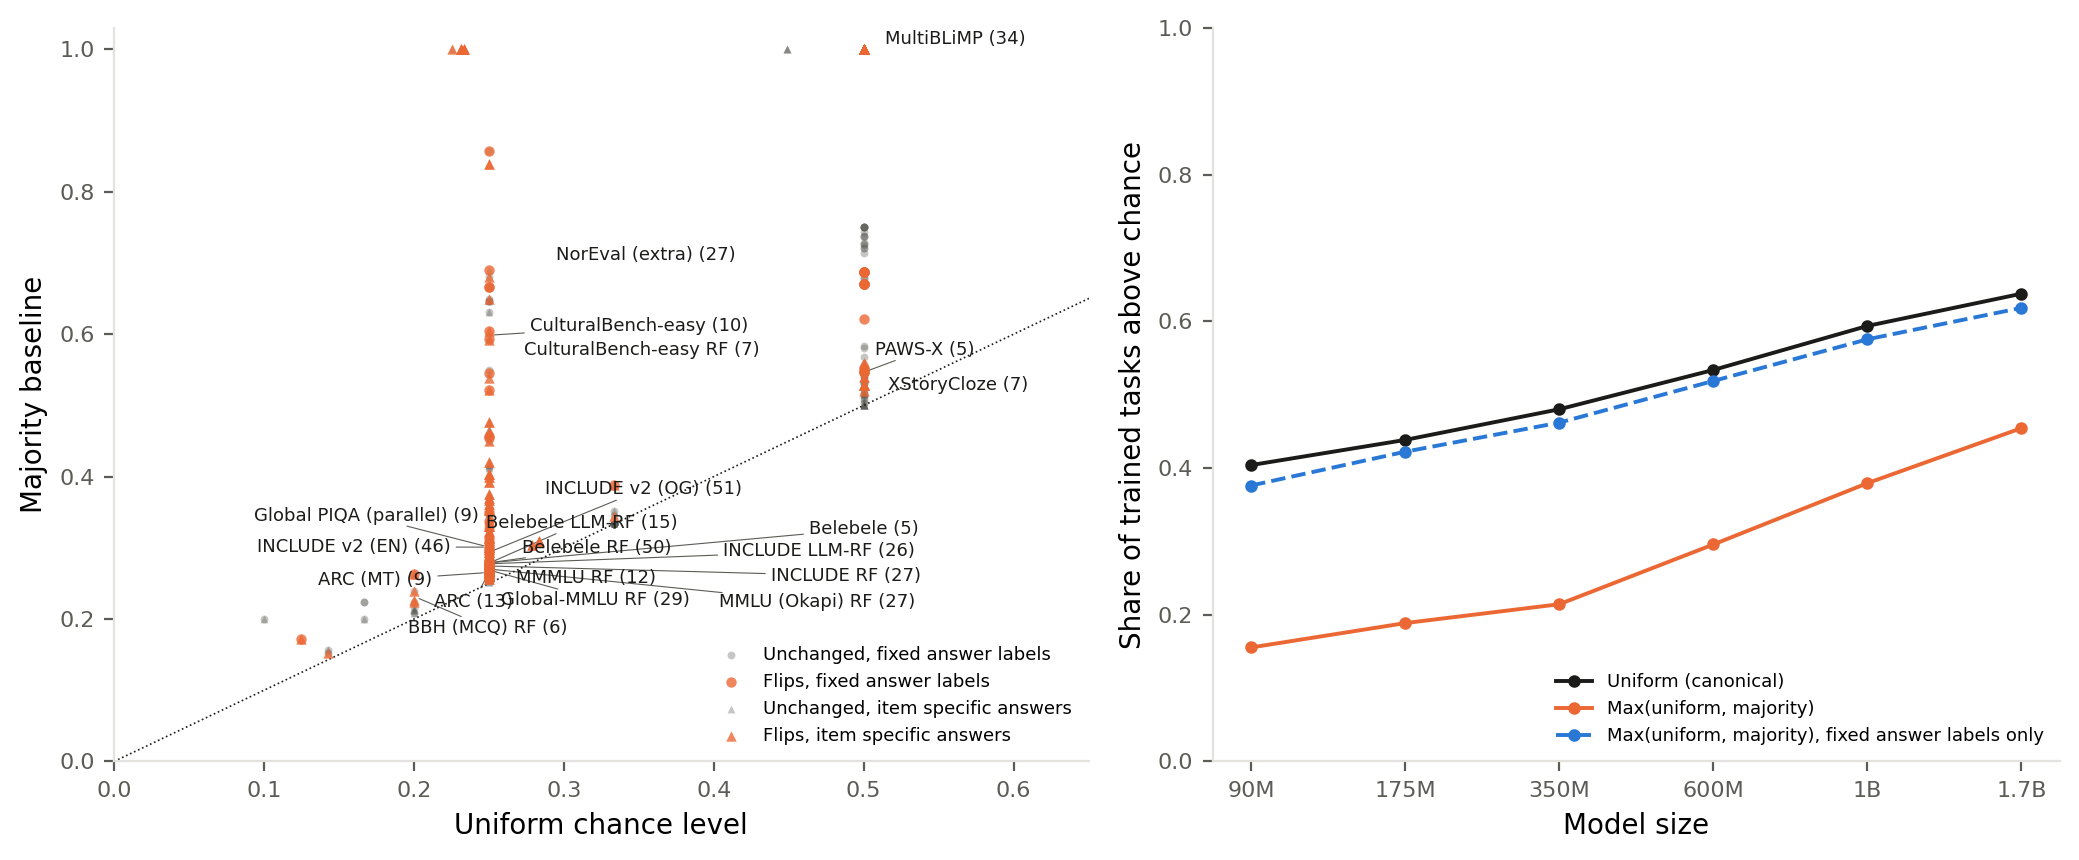
\includegraphics[width=\textwidth,height=0.8\textheight,keepaspectratio]{figures/app_rq00_majority_chance.png}
% source: src/signal-and-noise/analysis/rq00_gate_and_curves/majority_chance/majority_chance_paper.png
\caption{\textbf{A majority-class chance level removes passes mainly through answer order, which log-likelihood scoring cannot exploit.} The majority baseline of a task is the accuracy of always choosing its most frequent gold option position, read from the evaluated items. (a) Uniform chance against the majority baseline for the 933 trained tasks with a chance level. Orange marks the 447 tasks above chance at some size under the uniform level and at chance there under the larger of the two, with a benchmark label where a benchmark has at least five such tasks. Circles are tasks whose answer positions carry the same label on every item (a letter or a yes or no answer), where a model with a constant preference can reach the majority baseline. Triangles are tasks whose answers change per item. (b) Trained tasks above chance per size under the uniform level, under the majority level, and under the majority level applied to the labelled tasks only. Of the 933 trained tasks, 377 are above chance at 90M and 595 at 1.7B under the uniform level, 145 and 424 under the majority level, and 351 and 577 when only the labelled tasks change. Of the flipped tasks, 42 are labelled. Seed-1904 runs of every language setting, ladder and data build, with the Wilson rule of Appendix~\ref{app:chance-threshold}.}
\label{fig:app_rq00_majority_chance}
\end{figure*}
